\documentclass[12pt]{amsart}
\usepackage{amsmath,amsthm,amssymb,amsfonts,enumerate,mymath,tikz-cd,fancyhdr,multicol}
\openup 5pt
\author{Blake Farman\\University of South Carolina}
\title{Math 122\\Exam 03}
\date{April 13, 2017}
\pdfpagewidth 8.5in
\pdfpageheight 11in
\usepackage[margin=1in]{geometry}

\renewcommand{\qedsymbol}{}
\theoremstyle{definition}
\newtheorem{thm}{}
\newtheorem{lem}{Lemma}
\theoremstyle{definition}
\newtheorem{defn}{Definition}

\newcommand{\ddx}[1]{\frac{\operatorname{d}}{\operatorname{d}\!#1}}
\newcommand{\dx}[1]{\!\!\;\operatorname{d}\!#1}

\begin{document}
\maketitle

\begin{center}
  \fbox{\fbox{\parbox{5.5in}{\centering
        Answer the questions in the spaces provided on the
        question sheets and turn them in at the end of the class period.
        If you require extra space, use the back of the page and indicate that you have done so.
        
        Unless otherwise stated, all supporting work is required.
        Unsupported or otherwise mysterious answers will {\bf not receive credit.}
        You may use a calculator {\bf without a CAS} if you like, but a calculator is not necessary.
        By writing your name on the line below, you acknowledge that you have read and understand these directions.}}}
\end{center}

\vspace{0.2in}
\makebox[\textwidth]{Name:\enspace\hrulefill}
\vspace{0.2in}

$$
\begin{array}{|c|c|c||c|c|c|}
  \hline
  \text{Definitions} & \text{Points Earned} & \text{Points Possible} & \text{Problems} & \text{Points Earned} & \text{Points Possible}\\
  \hline
  1 & & 6 & 1 & & 20\\
  \hline
  2 & & 4 & 2 & & 12\\
  \hline
  3 & & 5 & 3 & & 8\\
  \hline
  4 & & 5 & 4 & & 15\\
  \hline
  5 & & 5 & 5 & & 20\\
  \hline
  \text{Subtotal} & & 25 & \text{Subtotal} & & 75\\
  \hline
  & & & \text{Total} & & 100\\
  \hline
\end{array}
$$

\newpage

\section{Definitions}

\begin{thm}[6 Points]
  If $F^\prime(t)$ is a continuous function on the interval $[a,b]$, then 
  $$\int_a^b F^\prime(t)\dx{t}\ =\ \line(1,0){250}$$
\end{thm}

\vspace{.15in}

\begin{thm}[4 Points]
  Assume that $\int f(x)\dx{x}$ and $\int g(x)\dx{x}$ exist.
  \begin{enumerate}[(a)]
  \item
    $$\int f(x) \pm g(x) \dx{x}\ =\ \line(1,0){250}$$
  \item
    Let $a$ be a number.
    $$\int af(x)\dx{x}\ =\ \line(1,0){250}$$
  \end{enumerate}
\end{thm}

\vspace{.15in}

\begin{thm}[5 Points]
  Let $n \neq 1$ be a fixed number.
  $$\int x^n \dx{x}\ =\ \line(1,0){250}$$
\end{thm}

\vspace{.15in}

\begin{thm}[5 Points]
  $$\int e^x \dx{x}\ =\ \line(1,0){250}$$
\end{thm}

\vspace{.15in}

\begin{thm}[5 Points]
  $$\int \frac{1}{x}\dx{x}\ =\ \line(1,0){250}$$
\end{thm}

\newpage

\section{Problems}
\setcounter{thm}{0}
\begin{thm}[20 Points]
  Compute the following indefinite integrals:
  \begin{enumerate}[(a)]
  \item
    $\displaystyle{\int 7 \dx{x}}$
    \vspace{1in}
  \item
    $\displaystyle{\int 10x + 2 \dx{x}}$
    \vspace{1in}
  \item
    $\displaystyle{\int 36x^2 + 26x \dx{x}}$
    \vspace{1in}
  \item
    $\displaystyle{\int x^2 \dx{x}}$
    \vspace{1in}
  \item
    $\displaystyle{\int \frac{1}{\sqrt{x}} \dx{x}}$
    \vspace{1in}
  \end{enumerate}
\end{thm}

\newpage
\begin{thm}[12 Points]
  Compute the following indefinite integrals.
  \begin{enumerate}[(a)]
  \item
    $\displaystyle{\int 25(x + 7)^{24} \dx{x}}$
    \vspace{2in}
  \item
    $\displaystyle{\int (x + 2)e^{\frac{1}{2}x^2 + 2x + 1}\dx{x}}$
    \vspace{2in}
  \item
    $\displaystyle{\int \frac{4x}{2x^2 + 7}\dx{x}}$
  \end{enumerate}
\end{thm}

\newpage
\begin{thm}[8 Points]
  Compute the following indefinite integrals.
\begin{enumerate}[(a)]
    \item
    $\displaystyle{\int \frac{x}{\sqrt{x^2 + 1}}\dx{x}}$
    \vspace{4in}
  \item
    $\displaystyle{\int 30e^{5x} - 2xe^{-x^2}\dx{x}}$
\end{enumerate}
\end{thm}

\newpage
\begin{thm}[15 Points]
  Consider the function $f$ given by the graph
  \begin{center}
    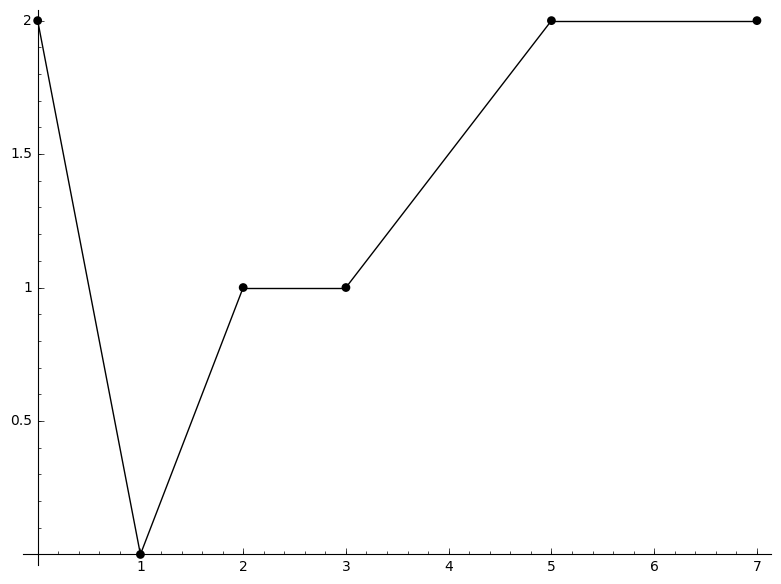
\includegraphics[scale=0.5]{imgs/geometricIntegral.png}
  \end{center}
  with marked points given by the table
  \begin{center}
    \begin{tabular}{c||cccccc}
      $x$ & 0 & 1 & 2 & 3 & 5 & 7\\
      \hline
      $f(x)$ & 2 & 0 & 1 & 1 & 2 & 2
    \end{tabular}
  \end{center}
  Compute $\displaystyle{\int_0^7 f(x)\dx{x}}$.
\end{thm}
\newpage

\begin{thm}[20 Points]
  Find the {\bf total} area between the graph of $x^3$ and the $x$-axis, between $x = -2$ and $x = 2$.
  That is, find the area of the shaded region below:
  \begin{center}
    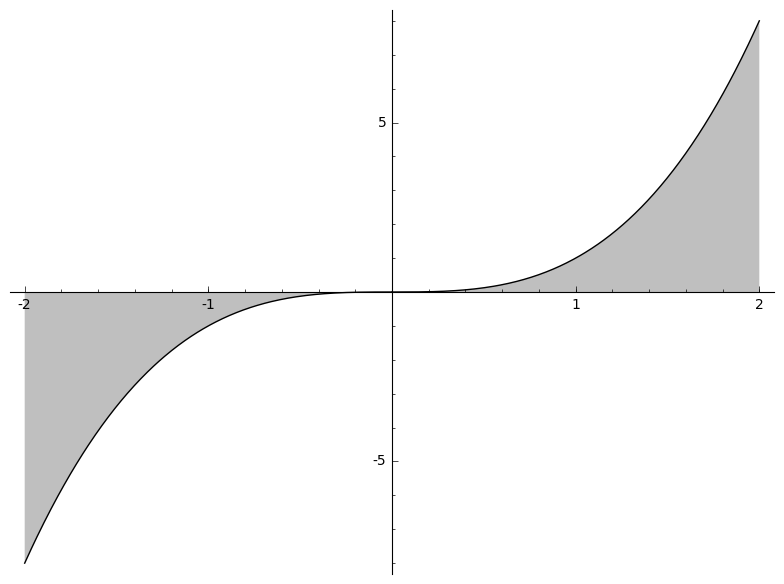
\includegraphics[scale=0.5]{imgs/areaBetweenCurves.png}
  \end{center}
\end{thm}

\end{document}
